\section{\ce{[Co(dca)_2(4-hydroxymethylpyridine)_2]_n}}
\subsection{Synthesis}
0.29 g \ce{Co(NO3)2*6 H2O} (1 mmol), 0.18 g sodium dicyanamide (2 mmol) and 0.22 g \ce{4-hydroxymethyl-pyridine} (2 mmol) were dissolved in 20 mL distilled \ce{ H2O}. The solution was heated up to 80$^\circ$C  and stirred for 2 hours and 30 minutes. After filtration the pink  solution was stirred at the same temperature for 40 minutes and then cooled down to RT. After 24 hours pink plate-like crystals were obtained.
Anal. Calculated for \ce{C_{16}H_{14}CoN_{8}O_{2}} (409.28 g/mol) : 46.96\% C; 3.45\% H; 27.38\% N;
Found: 46.76 \% C; 3.44\% H; 27.37 \% N;
IR (ATR, cm$^{-1}$): 3551(w), 3481 (w), 2269 (w), 2245 (m), 2170 (s), 1606 (m), 1564 (w), 1504 (w), 1426 (m), 1293 (s), 1202 (m), 1023 (vs), 799 (m), 607 (w), 533 (s), 493 (m)

\begin{figure}[h!]
\centering
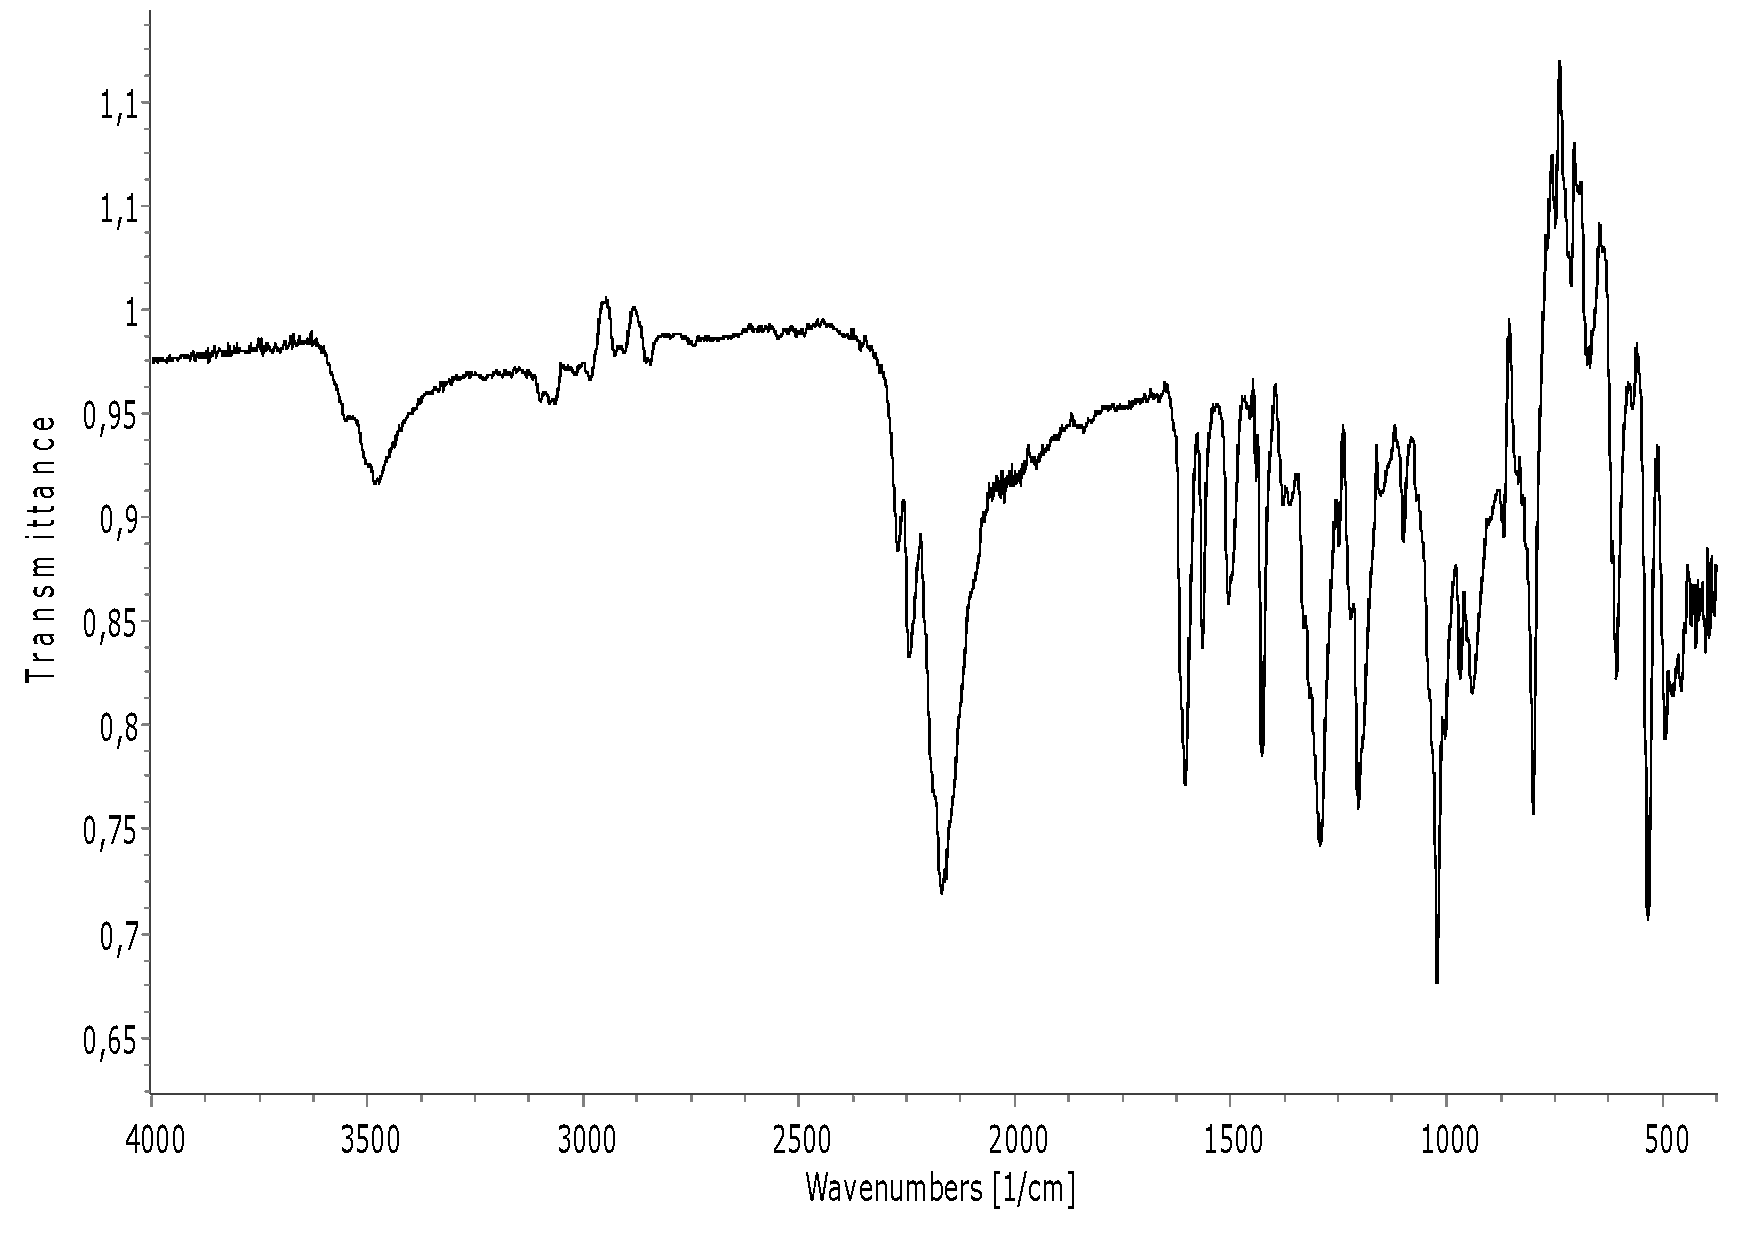
\includegraphics[width=1\textwidth]{figures/CoD4HOMP-IR.pdf}
\caption{IR spectrum of \ce{[Co(dca)_2(4-HOMepy)_2]_n}}
\end{figure}

\newpage


\subsection{Structural characterization}

A packing view  of \ce{[Co(dca)_2(4-HOMepy)_2]_n} is given in fig. \ref{fig:CoD4HOMP_packv} and a perspective view of a section of the polymeric chain  in fig. \ref{fig:CoD4HOMP_pv}. Selected bond parameters are summarized in table \ref{batab:CoD4HOMP}.  The Co(1) center is located on an inversion center. It is coordinated by pyridine N donor atom of two 4-MeOpy molecules in trans configuration and four N atoms of dicyanamide anions (acting in the bis-$\mu$(1,5)-bridging mode) generating polymeric chains of polyhedra. These are oriented along the c-axis of the monoclinic unit cell. The \ce{CoN6} chromophore has an almost regular octahedron, with Co-N bond distances varying from 2.116(4) to 2.126(4) \AA, and N-Co-N bond angles deviating only by 1.16$^\circ$ from the values of ideal octahedral geometry. The dca bridges possess the following bond parameters: Co-N-C: 163.3(4) and 158.5(4)$^\circ$; N-C-N: 177.0(5) and 176.5(
5)$^\circ$; C-N-C: 114.7(4)$^\circ$; C-N(nitril) 1.146(7) and 1.156(7) \AA; C-N(amide): 1.317(7) and 1.326(7) \AA. The intra-chain Co\ce{***}Co distance of 7.213(3) \AA\ \ is longer than the shortest inter-chain metal\ce{***}metal separation of 7.076(3) \AA. Along the a-axis of the unit cell the OH-group of the pyridine derivative ligand forms a hydrogen bond. This bond is  of  the type O-H\ce{***}N and is connected to the central N(3) atom of the adjacent dicyanamide anion (O(1)-H(90)\ce{***}N(3\#1) = 152(7)$^\circ$, O(1)ce{***}N(3\#1) = 2.954(7) \AA; (\#1): 1+x,y,z).



\renewcommand{\arraystretch}{1.2}
\begin{table}[htpb!]
\centering
\captionabove{Selected bond lengths (\AA) and angles ($^\circ$) for \ce{[Co(dca)_2(4-HOMepy)_2]_n}. Symmetry codes: (a) 1-x,1-y,-z; (b) 1-x,1-y,1-z; (c) -1+x,y,z; (d) x,y,1+z; (e) 1-x,1-y,-1-z. }
\begin{tabular}{|l|l|l|l|}
\hline
Co(1)-N(1a) & 2.126(4) & Co(1)-N(4a) & 2.124(5)\\
\hline
Co(1)-N(2a) & 2.116(4) & N(3)-C(7) & 1.317(7)\\
\hline
N(2)-C(7) & 1.146(7) & N(3)-C(8b) & 1.326(7)\\
\hline
N(4)-C(8) & 1.156(7) &  & \\
\hline
\hline
N(2)-Co(1)-N(4) & 90.34(17) & N(2a)-Co(1)-N(1a) & 91.16(17) \\
\hline
N(4)-Co(1)-N(1a) & 90.47(17) & N(2)-Co(1)-N(2a) & 180.0\\
\hline
Co(1)-N(2)-C(7) & 163.3(4) & N(2)-C(7)-N(3) & 177.0(5)\\
\hline
Co(1)-N(4)-C(8) & 158.5(4) & N(4)-C(8)-N(3b) & 176.5(5)\\
\hline
C(7)-N(3)-C(8b) & 114.7(4) &  & \\
\hline
\end{tabular}
\label{batab:CoD4HOMP}
\end{table}

\begin{figure}[htpb!]
\centering
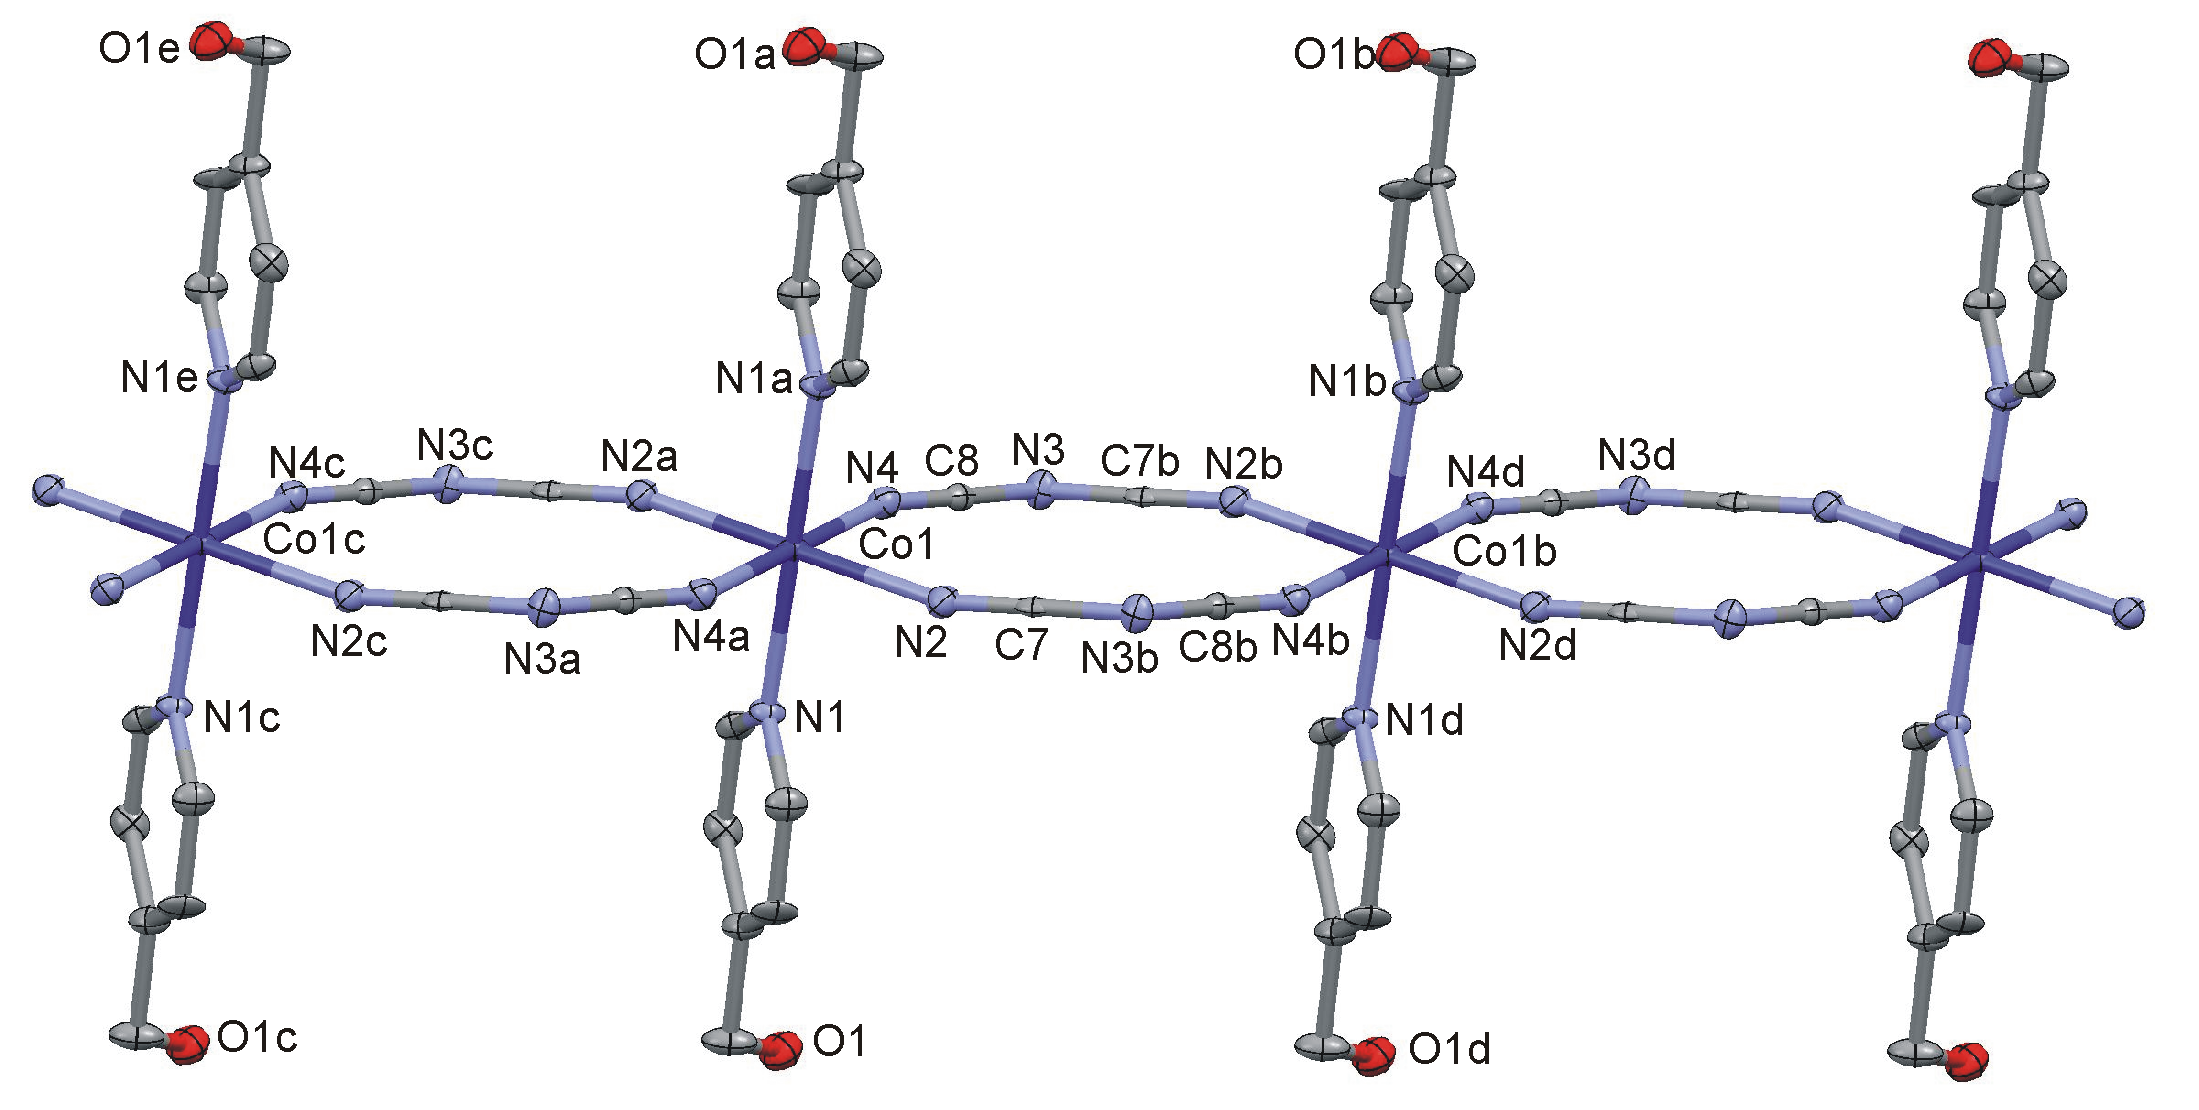
\includegraphics[width=1\textwidth]{figures/CoD_4OMP_FIGm11-1.png}
\caption[Perspective view of \ce{[Co(dca)_2(4-HOMepy)_2]_n}]{Perspective view of a section of the polymeric chain of \ce{[Co(dca)_2(4-HOMepy)_2]_n} together with the atom numbering scheme. Symmetry codes: (a) 1-x,1-y,-z; (b) 1-x,1-y,1-z; (c) -1+x,y,z; (d) x,y,1+z; (e) 1-x,1-y,-1-z.}
\label{fig:CoD4HOMP_pv}
\vspace{\floatsep}
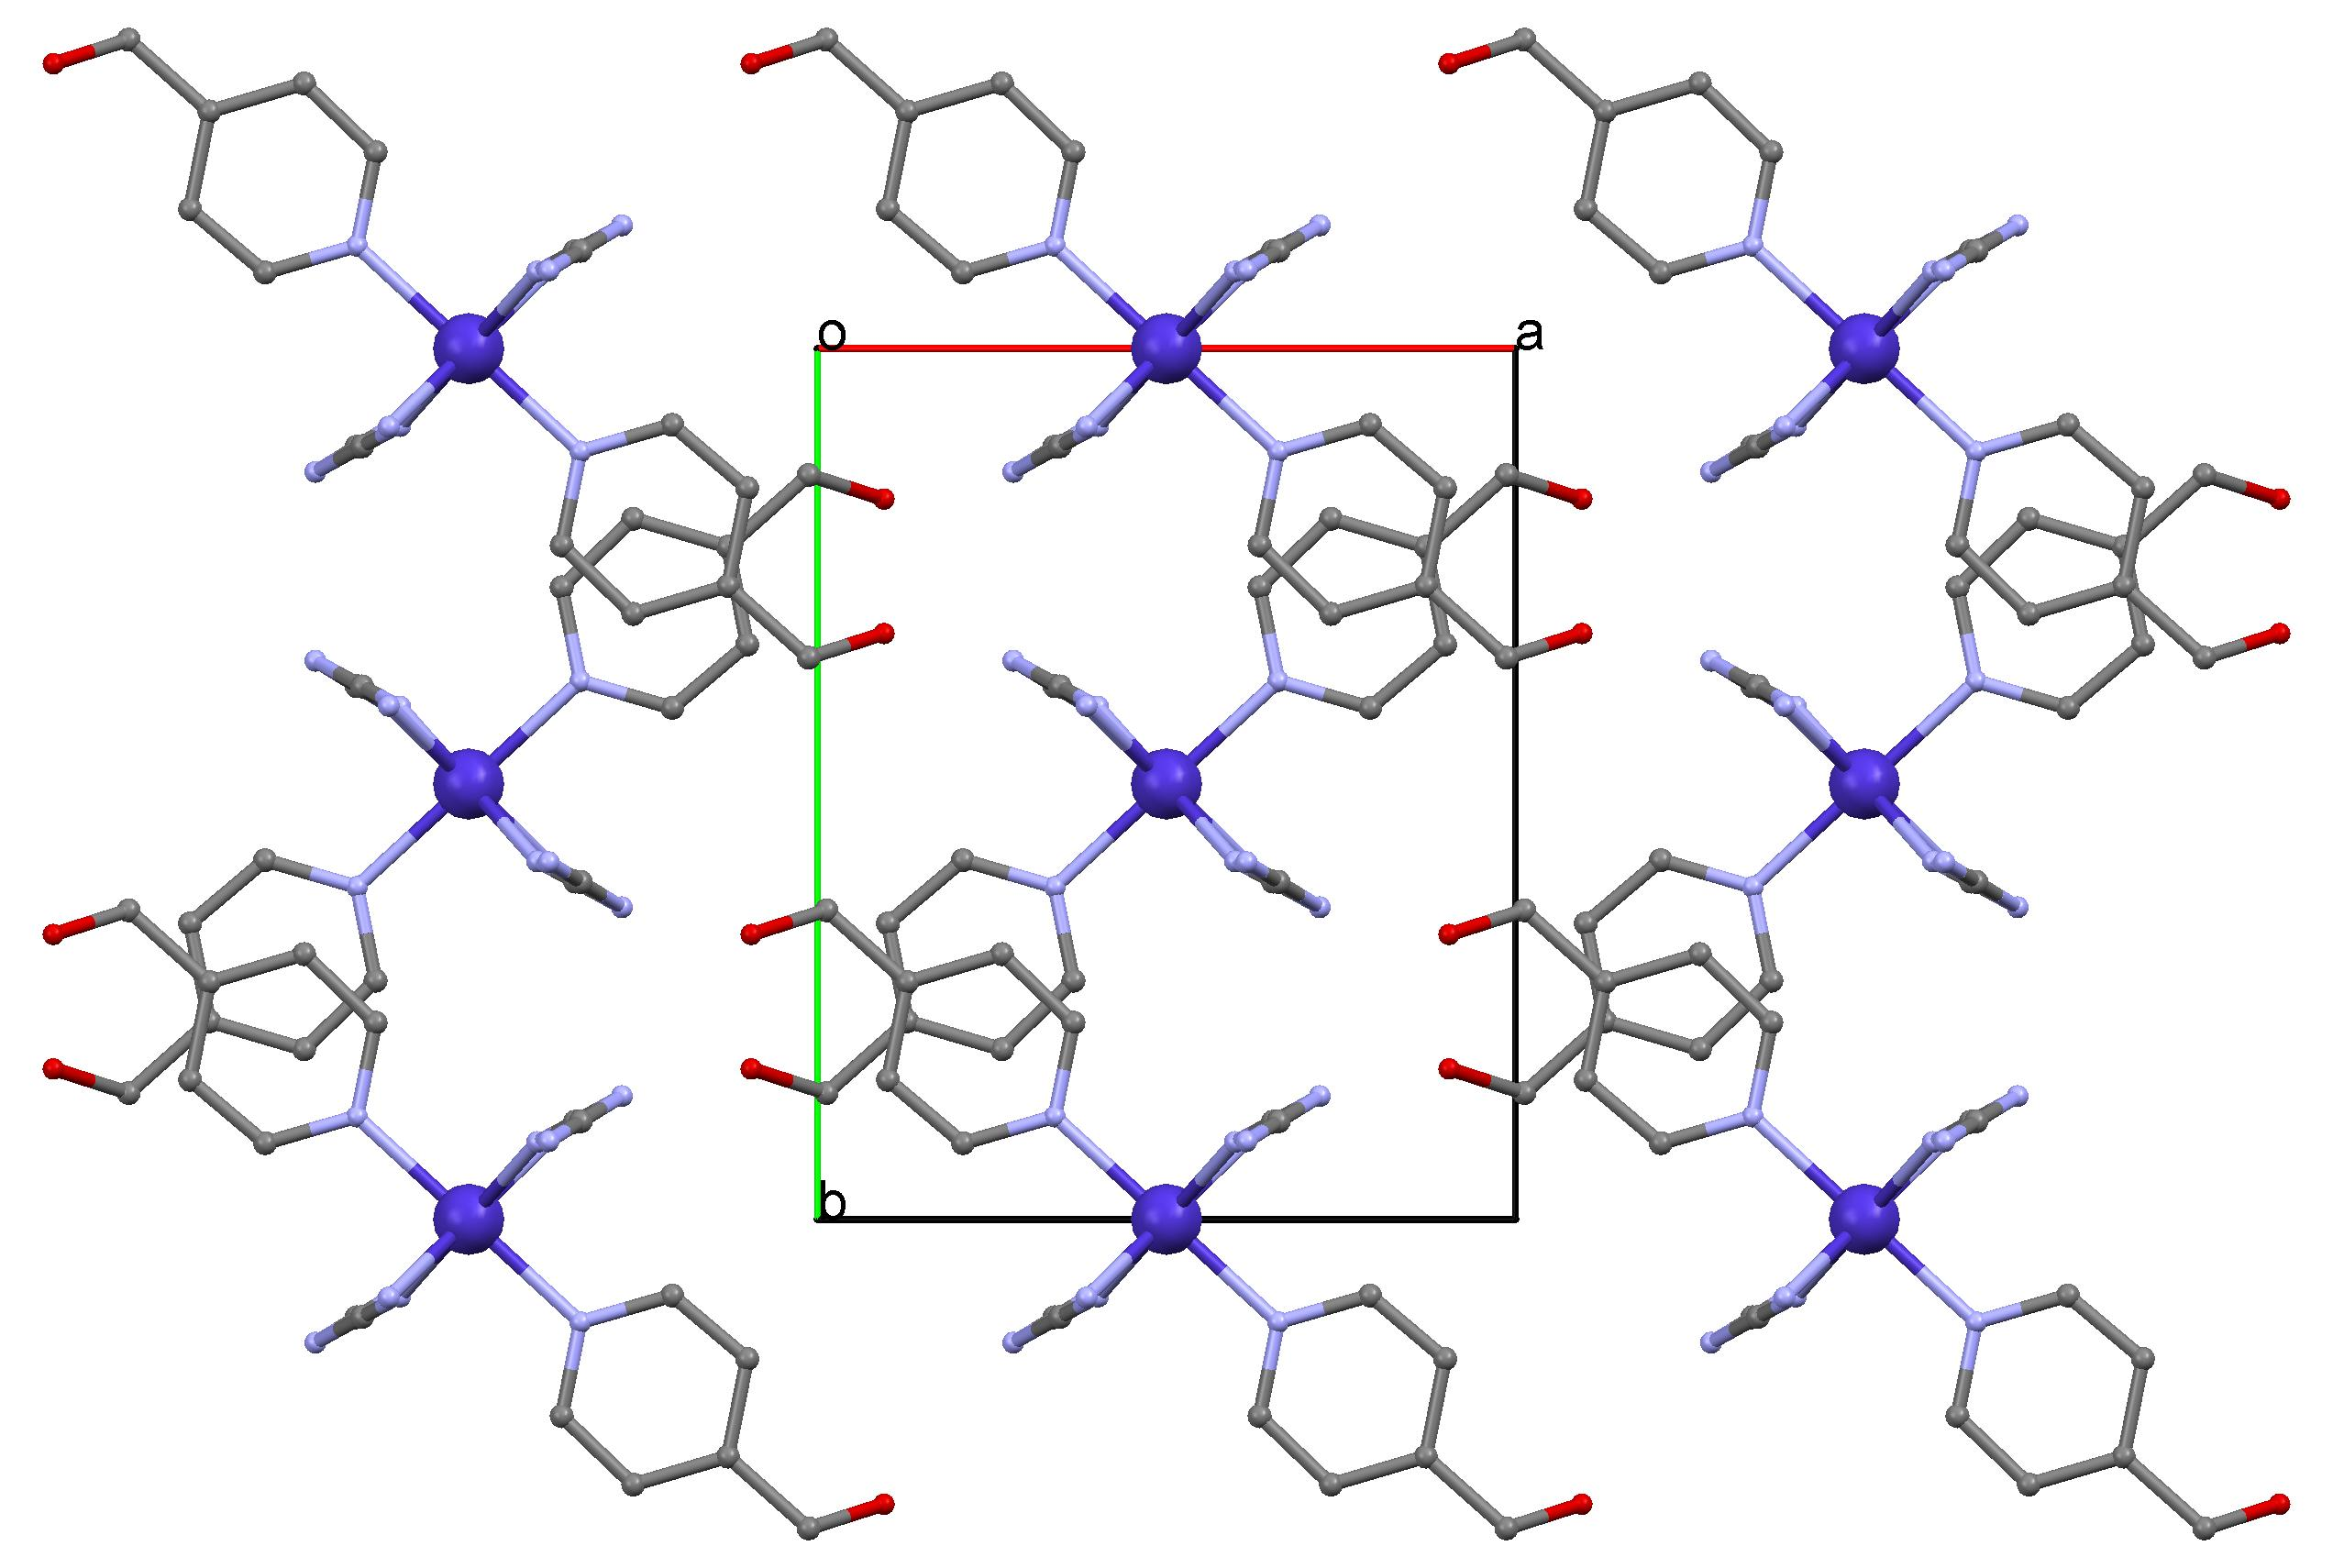
\includegraphics[width=1\textwidth]{figures/cod_4omp_CC-1.png}
\caption{Packing plot of \ce{[Co(dca)_2(4-HOMepy)_2]_n}.}
\label{fig:CoD4HOMP_packv}
\end{figure}





\renewcommand{\arraystretch}{1.5}
\begin{table}
\captionabove{Crystallographic data and processing parameter of \ce{[Co(dca)_2(4-HOMepy)_2]_n}}
\centering
\begin{tabular}{ | l |  l | }
\hline
Empirical formula & \ce{C_{16}H_{14}CoN_{8}O_{2}}\\
\hline
Formula mass & 409.28\\
\hline
System & monoclinic\\
\hline
Space group & P2$_1$/c\\
\hline
a ({\AA}) & 10.347(4)\\
\hline
b ({\AA}) & 12.175(5)\\
\hline
c ({\AA}) & 7.213(3)\\
\hline
$\alpha$ ($^\circ$) & 90\\
\hline
$\beta$ ($^\circ$) & 109.435(6)\\
\hline
$\gamma$ ($^\circ$) & 90\\
\hline
V (\AA$^{3}) $  & 856.9(6)\\
\hline
Z & 2\\
\hline
T (K) & 100(2)\\
\hline
$\mu$ (mm$^{-1}$) & 1.033\\
\hline
 D$_{calc}$ (Mg/m$^{3}$) & 1.586\\
\hline
Crystal size (mm) & 0.22 x 0.14 x 0.08\\
\hline
$\theta$ max ($^\circ$) & 26.34\\
\hline
Data collected & 6380\\
\hline
Unique refl./ R$_{int}$ & 1720 / 0.0474\\
\hline
Parameters & 127\\
\hline
Goodness-of-Fit on F$^{2}$ & 1.274\\
\hline
R1 / wR2 (all data) & 0.0814 /0.2004\\
\hline
Residual extrema (e/\AA$^{3}$) & 1.66 /-0.86\\
\hline
\end{tabular}

\label{ptab:CoD4HOMP}

\end{table}



